\scanpage{63}
% archive foliation: 62
$\unsure{\mathbb{E}\mathrm{xt}^*|\mathrm{Ext}^*}(X;M,N)$ est le \unsure{f\textsuperscript{r}} $\mathrm{Ext}$ dans la catégorie des motifs, i.e. ses foncteurs dérivés ?.

Pourtant, je doute que les $\mathrm{Ext}^i$ $(i>0)$ soient effaçables.....
\inserted{[\unsure{quid si on est} dans la catégorie des Ind-motifs ???]}
Notons la suite spectrale
\[
\mathbb{H}^*(X,M^\cdot)\Longleftarrow H^p(X,H^q(M^\cdot))
\]
d'où en particulier
\[
\unsure{\mathbb{E}\mathrm{xt}^*|\mathrm{Ext}^*}(X,M,N)\Longleftarrow H^p(X,\underline{\mathrm{Ext}}^q(M,N))
\]

4°) On veut \deleted{que \unsure{sous} des conditions \unsure{Naturelles}} \inserted{des hom de $\delta$-foncteurs}
\deleted{\unsure{sur} $X$}
\[
H^*(X,M)\deleted{\otimes_{\mathbf{Q}}\mathbf{Q}_\ell}\unsure{-|\longrightarrow} H^*(X,T_\ell(M))
\]
d'où aussi
\[
\mathrm{Ext}^*(X;M,N)\otimes_{\mathbf{Q}}\mathbf{Q}_\ell\longrightarrow \unsure{\mathbb{E}\mathrm{xt}^*|\mathrm{Ext}^*}(X;T_\ell(M),T_\ell(N))
\]
qui, \deleted{sous des conditions \unsure{d'annulation}} \inserted{sous l'hypothèse que $X$ est de type fini sur $\mathbf{Z}$}, \deleted{\unsure{sur} $X$} (\unsure{en avouant|en admettant} le fait que les seconds mbs sont de \unsure{t. f.} sur $\mathbf{Q}_\ell$)
\figure{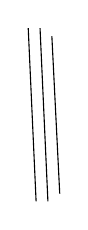
\begin{tikzpicture}[x=1mm,y=1mm]\draw (0,0)--(-1,22);\draw (1.5,0)--(0.5,22);\draw (3,1)--(2,21);\end{tikzpicture}}
